\newpage
\section{Módulo administrador}
En esta sección se muestran los casos de uso asociados al actor con el rol de administrador (ver figura \ref{fig:diagrama_cu_admin}).

\begin{figure}[h!]
    \centering
    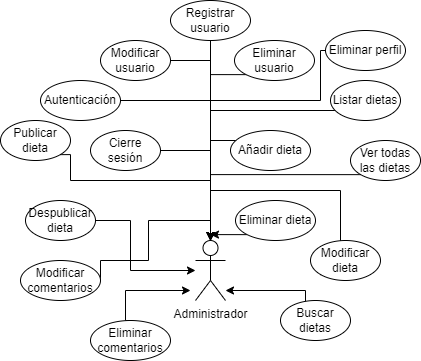
\includegraphics[width=0.75\textwidth]{Images/Capitulo4/cu-admin.png}
    \caption{Diagrama de casos de uso asociado al actor \textit{Administrador}}
    \label{fig:diagrama_cu_admin}
\end{figure}

%%%%%%%%%%%%%%%%%%%%%%%%
% TABLA 16
%%%%%%%%%%%%%%%%%%%%%%%%
\begin{table}[H]
\centering
\resizebox{\textwidth}{!}{%
\begin{tabular}{|l|l|}
\hline
\rowcolor[HTML]{8BC75F} 
\textbf{CU-32}         & \textbf{Registrar manualmente un usuario}\\ \hline
Descripción            & \begin{tabular}[c]{@{}l@{}}El administrador crea un usuario en el sistema con el rol de deportista\\ administrador\end{tabular}                                                                                                                                                   \\ \hline
Actor                  & Administrador                                                                                                                                                                                                                                                                     \\ \hline
Entrada                & Datos del usuario que se va a crear                                                                                                                                                                                                                                               \\ \hline
Salida                 & Mensaje de éxito o error                                                                                                                                                                                                                                                          \\ \hline
Origen                 & Vista de crear usuarios del administrador                                                                                                                                                                                                                                         \\ \hline
Precondición           & Tener una cuenta activa con el rol administrador                                                                                                                                                                                                                                  \\ \hline
Postcondición si éxito & El usuario se crea correctamente                                                                                                                                                                                                                                                  \\ \hline
Postcondición si fallo & \begin{tabular}[c]{@{}l@{}}Se vuelven a pedir los datos del nuevo usuario en el caso de haberse\\ producido un fallo\end{tabular}                                                                                                                                                 \\ \hline
Flujo normal           & \begin{tabular}[c]{@{}l@{}}1. El administrador hace click en el botón de crear usuario desde su\\ página principal\\ 2. Se introducen los datos requeridos para crear dicho usuario\\ 3. El usuario se crea satisfactoriamente con las credenciales\\ proporcionadas\end{tabular} \\ \hline
Flujo alternativo      & \begin{tabular}[c]{@{}l@{}}2. Se introduce algún dato clave ya existente, como el correo\\ electrónico\\ 3. Se muestra un mensaje de error y se vuelven a pedir los datos\end{tabular}                                                                                            \\ \hline

\end{tabular}%
}
\caption{Registrar manualmente un usuario}
\end{table}


%%%%%%%%%%%%%%%%%%%%%%%%
% TABLA 17
%%%%%%%%%%%%%%%%%%%%%%%%
\begin{table}[H]
\centering
\resizebox{\textwidth}{!}{%
\begin{tabular}{|l|l|}
\hline
\rowcolor[HTML]{8BC75F} 
\textbf{CU-33}         & \textbf{Modificar los datos de un usuario}\\ \hline
Descripción            & El administrador modifica los datos de un usuario del sistema                                                                                                                                                                                                                           \\ \hline
Actor                  & Administrador                                                                                                                                                                                                                                                                           \\ \hline
Entrada                & Nuevo datos del usuario que se va a crear                                                                                                                                                                                                                                               \\ \hline
Salida                 & Mensaje de éxito o error                                                                                                                                                                                                                                                                \\ \hline
Origen                 & Vista de modificar el perfil de un usuario                                                                                                                                                                                                                                              \\ \hline
Precondición           & El usuario que se quiere modificar debe existir en el sistema                                                                                                                                                                                                                           \\ \hline
Postcondición si éxito & Los datos del usuario son actualizados correctamente                                                                                                                                                                                                                                    \\ \hline
Postcondición si fallo & Se vuelven a pedir los nuevos datos del usuario                                                                                                                                                                                                                                         \\ \hline
Flujo normal           & \begin{tabular}[c]{@{}l@{}}1. El administrador hace click en el botón de todos los usuarios\\ desde su página principal\\ 2. Se accede al perfil del usuario que se quiera modificar\\ 3. Se editan los campos que sean necesarios\\ 4. Se pulsa sobre el botón de guardar\end{tabular} \\ \hline
Flujo alternativo      & \begin{tabular}[c]{@{}l@{}}3. Se introduce algún dato clave ya existente, como el correo\\ electrónico, y se muestra un mensaje de error\end{tabular}                                                                                                                                   \\ \hline

\end{tabular}%
}
\caption{Modificar los datos de un usuario}
\end{table}


%%%%%%%%%%%%%%%%%%%%%%%%
% TABLA 18
%%%%%%%%%%%%%%%%%%%%%%%%
\begin{table}[H]
\centering
\resizebox{\textwidth}{!}{%
\begin{tabular}{|l|l|}
\hline
\rowcolor[HTML]{8BC75F} 
\textbf{CU-34}         & \textbf{Eliminar a un usuario del sistema}\\ \hline
Descripción            & El administrador desactiva la cuenta de un usuario                                                                                                                                                                                                                                      \\ \hline
Actor                  & Administrador                                                                                                                                                                                                                                                                           \\ \hline
Entrada                & Identificador del usuario que se quiera desactivar                                                                                                                                                                                                                                      \\ \hline
Salida                 & Mensaje de éxito o error                                                                                                                                                                                                                                                                \\ \hline
Origen                 & Vista de modificar el perfil de un usuario                                                                                                                                                                                                                                              \\ \hline
Precondición           & El usuario que se quiere modificar debe existir en el sistema                                                                                                                                                                                                                           \\ \hline
Postcondición si éxito & Los datos del usuario son actualizados correctamente                                                                                                                                                                                                                                    \\ \hline
Postcondición si fallo & Se vuelven a pedir los nuevos datos del usuario                                                                                                                                                                                                                                         \\ \hline
Flujo normal           & \begin{tabular}[c]{@{}l@{}}1. El administrador hace click en el botón de todos los usuarios\\ desde su página principal\\ 2. Se accede al perfil del usuario que se quiera modificar\\ 3. Se editan los campos que sean necesarios\\ 4. Se pulsa sobre el botón de guardar\end{tabular} \\ \hline
Flujo alternativo      & \begin{tabular}[c]{@{}l@{}}3. Se introduce algún dato clave ya existente, como el correo\\ electrónico, y se muestra un mensaje de error\end{tabular}                                                                                                                                   \\ \hline

\end{tabular}%
}
\caption{Eliminar a un usuario del sistema}
\end{table}


%%%%%%%%%%%%%%%%%%%%%%%%
% TABLA 19
%%%%%%%%%%%%%%%%%%%%%%%%
\begin{table}[H]
\centering
\resizebox{\textwidth}{!}{%
\begin{tabular}{|l|l|}
\hline
\rowcolor[HTML]{8BC75F} 
\textbf{CU-35}         & \textbf{Autenticar administrador}\\ \hline

Descripción            & \begin{tabular}[c]{@{}l@{}}Etapa de inicio de sesión en la aplicación con el rol de \\ administrador.\end{tabular}                                                                                  \\ \hline
Actor                  & Administrador                                                                                                                                                                                       \\ \hline
Entrada                & Datos necesarios para el inicio de sesión                                                                                                                                                           \\ \hline
Salida                 & Mensaje de error o éxito                                                                                                                                                                            \\ \hline
Origen                 & Página de inicio de sesión                                                                                                                                                                          \\ \hline
Precondición           & Tener una cuenta creada y activa con ese correo                                                                                                                                                     \\ \hline
Postcondición si éxito & El administrador ha iniciado sesión correctamente                                                                                                                                                   \\ \hline
Postcondición si fallo & Se vuelven a pedir los datos de inicio de sesión                                                                                                                                                    \\ \hline
Flujo normal           & \begin{tabular}[c]{@{}l@{}}1. Se pulsa sobre el botón de login.\\ 2. Se introducen los datos de inicio de sesión\\ 3. Se comprueban los datos y si son correctos se inicia sesión\end{tabular} \\ \hline
Flujo alternativo      & \begin{tabular}[c]{@{}l@{}}3. Los datos introducidos no son correctos y se vuelve a la\\ página de inicio de sesión\end{tabular}    \\ \hline
\end{tabular}%
}
\caption{Autenticar administrador}
\end{table}


%%%%%%%%%%%%%%%%%%%%%%%%
% TABLA 20
%%%%%%%%%%%%%%%%%%%%%%%%
\begin{table}[H]
\centering
\resizebox{\textwidth}{!}{%
\begin{tabular}{|l|l|}
\hline
\rowcolor[HTML]{8BC75F} 
\textbf{CU-36}         & \textbf{Cerrar la sesión de un administrador}\\ \hline
Descripción            & El administrador cierra su sesión activa en la aplicación                                                                                                                                                               \\ \hline
Actor                  & Administrador                                                                                                                                                                                                           \\ \hline
Entrada                & NA                                                                                                                                                                                                                      \\ \hline
Salida                 & NA                                                                                                                                                                                                                      \\ \hline
Origen                 & Vista del perfil del administrador                                                                                                                                                                                      \\ \hline
Precondición           & El administrador debe existir y debe tener la sesión iniciada                                                                                                                                                           \\ \hline
Postcondición si éxito & Se cierra la sesión del administrador                                                                                                                                                                                   \\ \hline
Postcondición si fallo & La sesión del administrador no se ve alterada                                                                                                                                                                           \\ \hline
Flujo normal           & \begin{tabular}[c]{@{}l@{}}1. El administrador pulsa en el botón de ver perfil\\ 2. Se pulsa sobre las acciones del perfil en la parte superior derecha\\ 3. Se selecciona la opción de cerrar sesión\end{tabular} \\ \hline
Flujo alternativo      & NA                                                                                                                                                                                                                      \\ \hline

\end{tabular}%
}
\caption{Cerrar la sesión de un administrador}
\end{table}


%%%%%%%%%%%%%%%%%%%%%%%%
% TABLA 21
%%%%%%%%%%%%%%%%%%%%%%%%
\begin{table}[H]
\centering
\resizebox{\textwidth}{!}{%
\begin{tabular}{|l|l|}
\hline
\rowcolor[HTML]{8BC75F} 
\textbf{CU-37}         & \textbf{Añadir nueva dieta al sistema}\\ \hline
Descripción            & El administrador añade una nueva dieta al sistema                                                                                                                                                                                                                                    \\ \hline
Actor                  & Administrador                                                                                                                                                                                                                                                                        \\ \hline
Entrada                & Datos requeridos para crear una dieta                                                                                                                                                                                                                                                \\ \hline
Salida                 & Mensaje de éxito o error                                                                                                                                                                                                                                                             \\ \hline
Origen                 & Vista de crear una dieta                                                                                                                                                                                                                                                             \\ \hline
Precondición           & El administrador debe tener una cuenta activa en el sistema                                                                                                                                                                                                                          \\ \hline
Postcondición si éxito & La dieta se crea correctamente para ese usuario                                                                                                                                                                                                                                      \\ \hline
Postcondición si fallo & \begin{tabular}[c]{@{}l@{}}Se vuelven a pedir los datos de la dieta tras haber mostrado un\\ mensaje informando del fallo\end{tabular}                                                                                                                                               \\ \hline
Flujo normal           & \begin{tabular}[c]{@{}l@{}}1. El administrador pulsa sobre el botón de ver sus dietas creadas\\ 2. Se pulsa sobre el botón ``$+$`` en la parte inferior derecha\\ 3. Se introducen los datos requeridos de la dieta a crear\\ 4. Se pulsa sobre el botón de crear dieta\end{tabular} \\ \hline
Flujo alternativo      & \begin{tabular}[c]{@{}l@{}}3. El administrador no completa los campos requeridos para crear\\ una dieta\\ 4. Se muestra un mensaje de error y se vuelven a pedir los datos\end{tabular}                                                                                              \\ \hline

\end{tabular}%
}
\caption{El administrador crea una nueva dieta}
\end{table}


%%%%%%%%%%%%%%%%%%%%%%%%
% TABLA 22
%%%%%%%%%%%%%%%%%%%%%%%%
\begin{table}[H]
\centering
\resizebox{\textwidth}{!}{%
\begin{tabular}{|l|l|}
\hline
\rowcolor[HTML]{8BC75F} 
\textbf{CU-38}         & \textbf{Eliminar una dieta del sistema}\\ \hline

Descripción            & Eliminar una dieta del sistema                                                                                                                                                                                                             \\ \hline
Actor                  & Administrador                                                                                                                                                                                                                              \\ \hline
Entrada                & Identificador de la dieta que se quiere eliminar                                                                                                                                                                                           \\ \hline
Salida                 & Mensaje de error o éxito                                                                                                                                                                                                                   \\ \hline
Origen                 & \begin{tabular}[c]{@{}l@{}}Vista de la dieta que quieres eliminar\end{tabular}                                                                                           \\ \hline
Precondición           & \begin{tabular}[c]{@{}l@{}}Se ha iniciado sesión con una cuenta con el rol de administrador\\ y existe la dieta\end{tabular}                                                                                                               \\ \hline
Postcondición si éxito & Dieta eliminada correctamente                                                                                                                                                                                                              \\ \hline
Postcondición si fallo & Mensaje de error                                                                                                                                                                                                                           \\ \hline
Flujo normal           & \begin{tabular}[c]{@{}l@{}}1. Desde el menú principal se pulsa sobre el botón de todas las\\ dietas\\ 2. Se accede a la vista detalle de la dieta que quieres eliminar\\ 3. Se pulsa sobre el botón de eliminar\end{tabular} \\ \hline
Flujo alternativo      & 4. El usuario no acepta la confirmación de eliminar la dieta\\ \hline
\end{tabular}%
}
\caption{Eliminar una dieta del sistema}
\end{table}


%%%%%%%%%%%%%%%%%%%%%%%%
% TABLA 23
%%%%%%%%%%%%%%%%%%%%%%%%
\begin{table}[H]
\centering
\resizebox{\textwidth}{!}{%
\begin{tabular}{|l|l|}
\hline
\rowcolor[HTML]{8BC75F} 
\textbf{CU-39}         & \textbf{Modificar una dieta del sistema}\\ \hline

Descripción            & Se modifican algunos de los datos de una dieta                                                                                                                                                                                                                                                                                             \\ \hline
Actor                  & Administrador                                                                                                                                                                                                                                                                                                                              \\ \hline
Entrada                & Datos de la dieta que el administrador quiere modificar                                                                                                                                                                                                                                                                                    \\ \hline
Salida                 & Mensaje de error o éxito                                                                                                                                                                                                                                                                                                                   \\ \hline
Origen                 & Vista de la dieta que quieres modificar                                                                                                                                                                                                                                                                                                    \\ \hline
Precondición           & \begin{tabular}[c]{@{}l@{}}Se ha iniciado sesión con una cuenta con el rol de administrador\\ y existe la dieta\end{tabular}                                                                                                                                                                                                               \\ \hline
Postcondición si éxito & Dieta modificada con los nuevos datos introducidos previamente                                                                                                                                                                                                                                                                             \\ \hline
Postcondición si fallo & \begin{tabular}[c]{@{}l@{}}La dieta no ha sido modificada por lo que no se cambia ningún\\ dato\end{tabular}                                                                                                                                                                                                                               \\ \hline
Flujo normal           & \begin{tabular}[c]{@{}l@{}}1. Desde el menú principal se pulsa sobre el botón de todas las\\ dietas\\ 2. Se accede a la vista detalle de la dieta que quieres modificar\\ 3. Se pulsa sobre el botón de modificar.\\ 4. Se introducen los datos que se quieren modificar de la dieta\\ 5. Se pulsa sobre el botón de guardar\end{tabular} \\ \hline
Flujo alternativo      & 5. No se pulsa sobre el botón de guardar                                                                                                                                                                                                                                                                                                   \\ \hline

\end{tabular}%
}
\caption{Modificar una dieta del sistema}
\end{table}


%%%%%%%%%%%%%%%%%%%%%%%%
% TABLA 24
%%%%%%%%%%%%%%%%%%%%%%%%
\begin{table}[H]
\centering
\resizebox{\textwidth}{!}{%
\begin{tabular}{|l|l|}
\hline
\rowcolor[HTML]{8BC75F} 
\textbf{CU-40}         & \textbf{Publicar una dieta del sistema}\\ \hline
Descripción            & El administrador publica cualquier dieta sin publicar del sistema                                                                                                                                                    \\ \hline
Actor                  & Administrador                                                                                                                                                                                                        \\ \hline
Entrada                & Identificador de la dieta que se quiera publicar                                                                                                                                                                     \\ \hline
Salida                 & Mensaje de éxito o error                                                                                                                                                                                             \\ \hline
Origen                 & Vista detalle de la dieta que se quiera publicar                                                                                                                                                                     \\ \hline
Precondición           & \begin{tabular}[c]{@{}l@{}}El administrador debe tener una cuenta activa y la dieta debe existir\\ y estar despublicada\end{tabular}                                                                                 \\ \hline
Postcondición si éxito & La dieta es publicada y visible para todos los usuarios                                                                                                                                                              \\ \hline
Postcondición si fallo & El estado de publicación de la dieta no se ve alterado                                                                                                                                                               \\ \hline
Flujo normal           & \begin{tabular}[c]{@{}l@{}}1. El administrador pulsa sobre el botón de ver todas las dietas del sistema\\ 2. Se accede a la dieta que se quiera publicar\\ 3. Se pulsa sobre el botón de publicar dieta\end{tabular} \\ \hline
Flujo alternativo      & 3. El administrador no pulsa ningún botón de cambiar el estado de la dieta                                                                                                                                           \\ \hline
\end{tabular}%
}
\caption{Publicar una dieta del sistema}
\end{table}


%%%%%%%%%%%%%%%%%%%%%%%%
% TABLA 25
%%%%%%%%%%%%%%%%%%%%%%%%
\begin{table}[H]
\centering
\resizebox{\textwidth}{!}{%
\begin{tabular}{|l|l|}
\hline
\rowcolor[HTML]{8BC75F} 
\textbf{CU-41}         & \textbf{Despublicar una dieta del sistema}\\ \hline
Descripción            & El administrador despublica cualquier dieta publicada del sistema                                                                                                                                                                                                                \\ \hline
Actor                  & Administrador                                                                                                                                                                                                                                                                    \\ \hline
Entrada                & Identificador de la dieta que se quiera despublicar                                                                                                                                                                                                                              \\ \hline
Salida                 & Mensaje de éxito o error                                                                                                                                                                                                                                                         \\ \hline
Origen                 & Vista detalle de la dieta que se quiera despublicar                                                                                                                                                                                                                              \\ \hline
Precondición           & \begin{tabular}[c]{@{}l@{}}El administrador debe tener una cuenta activa y la dieta debe existir\\ y estar publicada\end{tabular}                                                                                                                                                \\ \hline
Postcondición si éxito & La dieta es despublicada y deja de ser visible para todos los usuarios                                                                                                                                                                                                           \\ \hline
Postcondición si fallo & El estado de publicación de la dieta no se ve alterado                                                                                                                                                                                                                           \\ \hline
Flujo normal           & \begin{tabular}[c]{@{}l@{}}1. El administrador pulsa sobre el botón de ver todas las dietas del sistema\\ o sobre el botón de dietas publicadas en el sistema\\ 2. Se accede a la dieta que se quiera despublicar\\ 3. Se pulsa sobre el botón de despublicar dieta\end{tabular} \\ \hline
Flujo alternativo      & 3. El administrador no pulsa ningún botón de cambiar el estado de la dieta                                                                                                                                                                                                       \\ \hline

\end{tabular}%
}
\caption{Despublicar una dieta del sistema}
\end{table}


%%%%%%%%%%%%%%%%%%%%%%%%
% TABLA 26
%%%%%%%%%%%%%%%%%%%%%%%%
\begin{table}[H]
\centering
\resizebox{\textwidth}{!}{%
\begin{tabular}{|l|l|}
\hline
\rowcolor[HTML]{8BC75F} 
\textbf{CU-42}         & \textbf{Modificar comentarios de una dieta}\\ \hline

Descripción            & Se modifican los comentarios de una dieta                                                                                                                                                                                                                                                                                                               \\ \hline
Actor                  & Administrador                                                                                                                                                                                                                                                                                                                                           \\ \hline
Entrada                & Comentario que se quiere modificar sobre la dieta                                                                                                                                                                                                                                                                                                       \\ \hline
Salida                 & Mensaje de éxito                                                                                                                                                                                                                                                                                                                                        \\ \hline
Origen                 & \begin{tabular}[c]{@{}l@{}}Vista de todos los comentarios de la dieta seleccionada\\ previamente\end{tabular}                                                                                                                                                                                                                                           \\ \hline
Precondición           & \begin{tabular}[c]{@{}l@{}}Se ha iniciado sesión con una cuenta con el rol de administrador\\ y existe la dieta\end{tabular}                                                                                                                                                                                                                            \\ \hline
Postcondición si éxito & Dieta modificada con los comentarios modificados previamente                                                                                                                                                                                                                                                                                            \\ \hline
Postcondición si fallo & \begin{tabular}[c]{@{}l@{}}Los comentarios de la dieta no han sido modificados por lo que \\ no se actualiza ningún comentario\end{tabular}                                                                                                                                                                                                             \\ \hline
Flujo normal           & \begin{tabular}[c]{@{}l@{}}1. Desde el menú principal se pulsa sobre el botón de todas las\\ dietas.\\ 2. Se accede a la vista detalle de la dieta que quieres actualizar \\ el comentario\\ 3. Se pulsa sobre el botón de comentarios\\ 4. Se actualiza el comentario de la dieta especificada\\ 5. Se pulsa sobre el botón de actualizar\end{tabular} \\ \hline
Flujo alternativo      & 5. No se pulsa sobre el botón de actualizar                                                                                                                                                                                                                                                                                                             \\ \hline

\end{tabular}%
}
\caption{Modificar comentarios de una dieta}
\end{table}

%%%%%%%%%%%%%%%%%%%%%%%%
% TABLA 27
%%%%%%%%%%%%%%%%%%%%%%%%
\begin{table}[H]
\centering
\resizebox{\textwidth}{!}{%
\begin{tabular}{|l|l|}
\hline
\rowcolor[HTML]{8BC75F} 
\textbf{CU-43}         & \textbf{Eliminar comentarios de una dieta}\\ \hline
Descripción            & El administrador elimina un comentario de una dieta publicada                                                                                                                                                                                                                                      \\ \hline
Actor                  & Administrador                                                                                                                                                                                                                                                                                      \\ \hline
Entrada                & Identificador del comentario que se quiera eliminar                                                                                                                                                                                                                                                \\ \hline
Salida                 & Mensaje de éxito o error                                                                                                                                                                                                                                                                           \\ \hline
Origen                 & Vista detalle de los comentarios de la dieta publicada                                                                                                                                                                                                                                             \\ \hline
Precondición           & \begin{tabular}[c]{@{}l@{}}El administrador debe tener una cuenta activa y la dieta debe existir, estar\\ publicada y tener al menos un comentario que eliminar\end{tabular}                                                                                                                       \\ \hline
Postcondición si éxito & El comentario es borrado de la dieta publicada                                                                                                                                                                                                                                                     \\ \hline
Postcondición si fallo & El comentario no es eliminado                                                                                                                                                                                                                                                                      \\ \hline
Flujo normal           & \begin{tabular}[c]{@{}l@{}}1. El administrador pulsa sobre el botón de ver todas las dietas publicadas\\ 2. Se accede a la dieta que tiene el comentario que se quiera borrar\\ 3. Se pulsa sobre el botón de comentarios\\ 4. En las opciones del comentario se pulsa sobre eliminar\end{tabular} \\ \hline
Flujo alternativo      & 4. El administrador no pulsa ningún botón de las acciones del comentario                                                                                                                                                                                                                           \\ \hline
\end{tabular}%
}
\caption{Eliminar comentarios de una dieta}
\end{table}



%%%%%%%%%%%%%%%%%%%%%%%%
% TABLA 29
%%%%%%%%%%%%%%%%%%%%%%%%
\begin{table}[H]
\centering
\resizebox{\textwidth}{!}{%
\begin{tabular}{|l|l|}
\hline
\rowcolor[HTML]{8BC75F} 
\textbf{CU-44}         & \textbf{Eliminar perfil de un administrador}\\ \hline
Descripción            & Se elimina la cuenta del administrador                                                                                                                                                                                                        \\ \hline
Actor                  & Administrador                                                                                                                                                                                                                                 \\ \hline
Entrada                & Confirmación del usuario                                                                                                                                                                                                                   \\ \hline
Salida                 & Mensaje de éxito o error si se ha borrado el perfil satisfactoriamente                                                                                                                                                                     \\ \hline
Origen                 & Vista del perfil del administrador                                                                                                                                                                                                            \\ \hline
Precondición           & El usuario debe tener una cuenta activa y debe de haber iniciado sesión                                                                                                                                                                    \\ \hline
Postcondición si éxito & Se elimina la cuenta del usuario del sistema                                                                                                                                                                                               \\ \hline
Postcondición si fallo & La cuenta del administrador no se ve alterada                                                                                                                                                                                                 \\ \hline
Flujo normal           & \begin{tabular}[c]{@{}l@{}}1. Se accede desde el menú principal al perfil del usuario\\ 2. Se pulsa sobre las opciones del perfil\\ 3. Se selecciona la opción de eliminar cuenta\\ 4. Se elimina la cuenta del administrador tras la confirmación\end{tabular} \\ \hline
Flujo alternativo      & 4. El administrador deniega la confirmación de borrar cuenta y no sucede nada                                                                                                                                                                 \\ \hline

\end{tabular}%
}
\caption{Eliminar perfil de un administrador}
\end{table}

%%%%%%%%%%%%%%%%%%%%%%%%
% TABLA 30
%%%%%%%%%%%%%%%%%%%%%%%%
\begin{table}[H]
\centering
\resizebox{\textwidth}{!}{%
\begin{tabular}{|l|l|}
\hline
\rowcolor[HTML]{8BC75F} 
\textbf{CU-45}         & \textbf{Listar dietas creadas por del administrador}\\ \hline
Descripción            & Se muestran todas las dietas que el administrador ha creado                                                                                                                 \\ \hline
Actor                  & Administrador                                                                                                                                                               \\ \hline
Entrada                & Identificador del administrador                                                                                                                                                \\ \hline
Salida                 & Todas las dietas del administrador                                                                                                                                             \\ \hline
Origen                 & Vista de ver todas las dietas                                                                                                                                            \\ \hline
Precondición           & El administrador debe tener una cuenta activa en el sistema                                                                                                                    \\ \hline
Postcondición si éxito & Se muestran todas las dietas que el administrador ha creado                                                                                                                    \\ \hline
Postcondición si fallo & NA                                                                                                                                                                       \\ \hline
Flujo normal           & \begin{tabular}[c]{@{}l@{}}1. Desde la página principal se pulsa sobre el botón de dietas creadas\\ 2. Todas las dietas creadas por el administrador son listadas\end{tabular} \\ \hline
Flujo alternativo      & NA                                                                                                                                                                       \\ \hline

\end{tabular}%
}
\caption{Listar dietas creadas por del administrador}
\end{table}

%%%%%%%%%%%%%%%%%%%%%%%%
% TABLA 12
%%%%%%%%%%%%%%%%%%%%%%%%
\begin{table}[H]
\centering
\resizebox{\textwidth}{!}{%
\begin{tabular}{|l|l|}
\hline
\rowcolor[HTML]{8BC75F} 
\textbf{CU-46}         & \textbf{Ver todas las dietas del sistema}\\ \hline
Descripción            & Se muestran todas las dietas del sistema                                                                                                                           \\ \hline
Actor                  & Administrador                                                                                                                                                                    \\ \hline
Entrada                & NA                                                                                                                                                                            \\ \hline
Salida                 & Todas las dietas  que hay en el sistema                                                                                                                             \\ \hline
Origen                 & Vista de todas las dietas publicadas                                                                                                                                          \\ \hline
Precondición           & Tiene que haber dietas que los usuarios hayan creado                                                                                                                       \\ \hline
Postcondición si éxito & Se muestran todas las dietas en formato tabla                                                                                                                      \\ \hline
Postcondición si fallo & NA                                                                                                                                                                            \\ \hline
Flujo normal           & \begin{tabular}[c]{@{}l@{}}1. Desde la página principal se pulsa sobre el botón de todas las dietas \\ 2. Todas las dietas en el sistema son listadas\end{tabular} \\ \hline
Flujo alternativo      & NA                                                                                                                                                                            \\ \hline

\end{tabular}%
}
\caption{Ver todas las dietas publicadas del sistema}
\end{table}

%%%%%%%%%%%%%%%%%%%%%%%%
% TABLA 13
%%%%%%%%%%%%%%%%%%%%%%%%
\begin{table}[H]
\centering
\resizebox{\textwidth}{!}{%
\begin{tabular}{|l|l|}
\hline
\rowcolor[HTML]{8BC75F} 
\textbf{CU-47}         & \textbf{Buscar dietas}\\ \hline
Descripción            & El administrador busca una dieta entre todas las dietas                                                                                                                                                                                                      \\ \hline
Actor                  & Administrador                                                                                                                                                                                                                                                          \\ \hline
Entrada                & Texto introducido por el administrador sobre el que buscar dietas                                                                                                                                                                                                         \\ \hline
Salida                 & \begin{tabular}[c]{@{}l@{}}Todas las dietas cuyos títulos coinciden de cierta forma\\ con el texto introducido\end{tabular}                                                                                                                              \\ \hline
Origen                 & Vista de todas las dietas                                                                                                                                                                                                                                 \\ \hline
Precondición           & Tiene que haber dietas en el sistema                                                                                                                                                                                                                     \\ \hline
Postcondición si éxito & \begin{tabular}[c]{@{}l@{}}Se muestran todas las dietas con un título similar al texto\\ introducido\end{tabular}                                                                                                                                        \\ \hline
Postcondición si fallo & No se muestra ninguna dieta en la tabla de la correspondiente vista                                                                                                                                                                                                 \\ \hline
Flujo normal           & \begin{tabular}[c]{@{}l@{}}1. Desde la página principal se pulsa sobre el botón de ver todas las dietas\\ 2. Se escribe el texto deseado sobre la barra superior de búsqueda\\ 3. Se listan todas las dietas cuyos títulos coinciden con el texto buscado\end{tabular} \\ \hline
Flujo alternativo      & \begin{tabular}[c]{@{}l@{}}3. No hay dietas que coincidan con el texto de la búsqueda y por lo tanto\\ ninguna dieta es listada\end{tabular}                                                                                                                        \\ \hline

\end{tabular}%
}
\caption{Buscar dietas}
\end{table}
